\documentclass[12pt]{article}

\usepackage[section]{algorithm}
\usepackage{algorithmic}
\usepackage{amsmath}
\usepackage{booktabs}
\usepackage{cite}
\usepackage{graphicx}
\usepackage{algorithm}
\usepackage{algorithmic}
\usepackage{latexsym}
\usepackage{multirow}

\title{Title}
\author{Andrew Mason \and Jonathan Pfeil}

\begin{document}
\maketitle
\tableofcontents
\listofalgorithms
\pagebreak

\section{Introduction}
\section{Background}
\subsection{Semantic Representation}

Abstract Meaning Representation (AMR)\cite{amr_sembank} attempts to unify the
semantic representation of natural language sentences. Unlike syntactic
annotations, semantic annotations often differ for different semantic relations
(named entities, temporal entities, co-referencing, etc). AMR, by contrast,
provides a single, graphical representation of the logical meaning of a
sentence, which can be easily understood by both humans and computers.

An AMR-annotated sentence is directed, rooted, labeled graph, or as a
conjunction of logical triples. Throughout this paper, we work with the AMRs
exclusively in the graphical form $G=(V,E)$, and will thus refer to the AMR
using just the sets $V,E$.

\subsection{Discourse Planning}

In Reiter and Dale's {\em Building Applied Natural Language Generation Systems}, they outline a 6-module pipeline for an NLG system. The second task in this system is Discourse Planning, which they describe as the process of imposing ordering and structure over the set of messages to be conveyed \cite{applied_nlg}. The order of pieces of information in text is not random; rather authors impose a structure on the messages for reasons such as: making the text easier to understand, highlighting the relationships between messages in the text, or stylistic preferences.When making an argument, authors must order the messages so that readers can see the logical implications from one message to the next; if the ordering of the messages were scrambled, readers may fail to understand the argument, even though the same set of information was communicated.

In addition to just logical implication, adjacent sentences can have many different types of relationships with each other, referred to as {\em discourse relations}. A commonly used set of discourse relations are those proposed by {\em Rhetorical Structure Theory} (RST) \cite{rst}. RST defines 32 discourse relations across 3 categories: ``Presentational Relations'', ``Subject Matter Relations'', and ``Multinuclear Relations''.

In applied systems, discourse planning is usually implemented through either schema-based systems or AI planning systems \cite{applied_nlg}. In schema-based systems, messages are given class labels, and are substituted into the appropriate slots which have been predefined in each schema. AI planning is a more general solution in which planning operators are associated with discourse relations, and then off-the-shelf planners can be used to construct a valid discourse plan \cite{hovy1993automated}\cite{paris1990natural}.

\subsection{Information Ordering}

Information ordering is an integral component of the Discourse Planning phase
of the NLG pipeline, discussed above and in \cite{applied_nlg}. After an
information set has been structured into to pieces of information (``facts" or
sentences), these pieces need to be ordered so that the reader can process and
understand the information being conveyed as easily as possible. This is often
approached as a planning problem, though Dimitromanolaki and
Androutsopoulos\cite{learning_to_order_facts} explore using pipelined decision
trees and instance-based learning.

\section{Related Work}

Early work by Kukich described a system for ``knowledge-based report generation'' in which manually specified domain rules were used to merge database facts into higher level messages, which were then ordered by a discourse module \cite{kukich1983knowledge}. The ordered output could later be passed to generation system to build a report. Work by Paris in 1990 and Hovy in 1993 introduced the idea of using AI Planners to generate discourse plans. They focused on finding explicit discourse relations between messages and using planners to generate an ordering which was allowed under the constraints of the discourse relations identified \cite{paris1990natural}\cite{hovy1993automated}. More recently, Duboue and Mckeown applied Machine Learning (ML) approaches to discourse planning. In \cite{duboue2001empirically}, they present an algorithm to learn ordering constraints among facts. In \cite{duboue2002content}, they build upon this work, using evolutionary algorithms to learn the tree representation of a planner. Although these systems seek to generate valid discourse plans, they do not use a scoring function to choose the `best' among the many valid plans that are available. Dimitromanolaki and Androutsopoulos used ML techniques to learn such a scoring function \cite{learning_to_order_facts}. They train a pipeline of classifiers that repeatedly choose the next fact to be added to a paragraph for a specific domain.
In order to train this pipeline, Dimitromanolaki and Androutsopoulos assume a
fixed $k$ number of sentences per paragraph (in their paper $k=6$).

Our work differs from this prior research in four major ways: (1) It is strictly at a semantic level. Our entire pipeline is built upon AMR semantics, rather than natural language `facts', meaning the internal entities and their relations can be reasoned about. (2) Higher-level messages are constructed as part of the discourse planning process. While other systems work at the individual fact level, our system seeks to group facts into higher level sentential messages that are ordered by our discourse module. The order of sentential units should be dependent on the information they contain, therefore the merging procedure must occur before or during the discourse planning. (3) Our system does not explicitly model the discourse relations between units.
(4) Our system imposes no limit on the number of sentences in a given
paragraph.

\section{Data}

The dataset for this research was the AMR ``proxy" dataset - a corpus of
AMR-annotated sentences obtained from newswire data. Since the source text of
the articles was unavailable, we used a sliding window approach to generate
``paragraphs" of size $k$ from the articles. For an article with $n$ sentences,
we could generate paragraphs containing sentences $(s_1,s_2,\ldots,s_k),
(s_2,s_3,\ldots,s_k,s_{k+1}), \ldots (s_{n-k},s_{n-k+1},\ldots,s_n)$.
As an example from our dataset, ``A prosecutor in South Korea seized 80
kilograms of drugs'' would have the following first-order logical form and AMR
representation.\\

\noindent \textbf{Logical form}:
\begin{equation}
\begin{split}
\exists s,d2,p2,c,n: &\\
&\text{instance}(s,want\text{-}01) \wedge \text{instance}(d2, drug) \wedge \\
&\text{instance}(p2, prosecutor) \wedge \text{instance}(c, country) \wedge \\
&\text{instance}(n, name) \wedge \text{arg0}(s,p2) \wedge \text{arg1}(s,d2)
\wedge \\ &\text{arg2}(s,c) \wedge \text{name}(c,n) \wedge \text{op1}(n,
``South") \wedge \\ &\text{op2}(n, ``Korea") \wedge \text{unit}(d2, kilogram)
\wedge \text{quant}(d2, 80)
\end{split}
\end{equation}
\textbf{AMR form}:
\begin{figure}
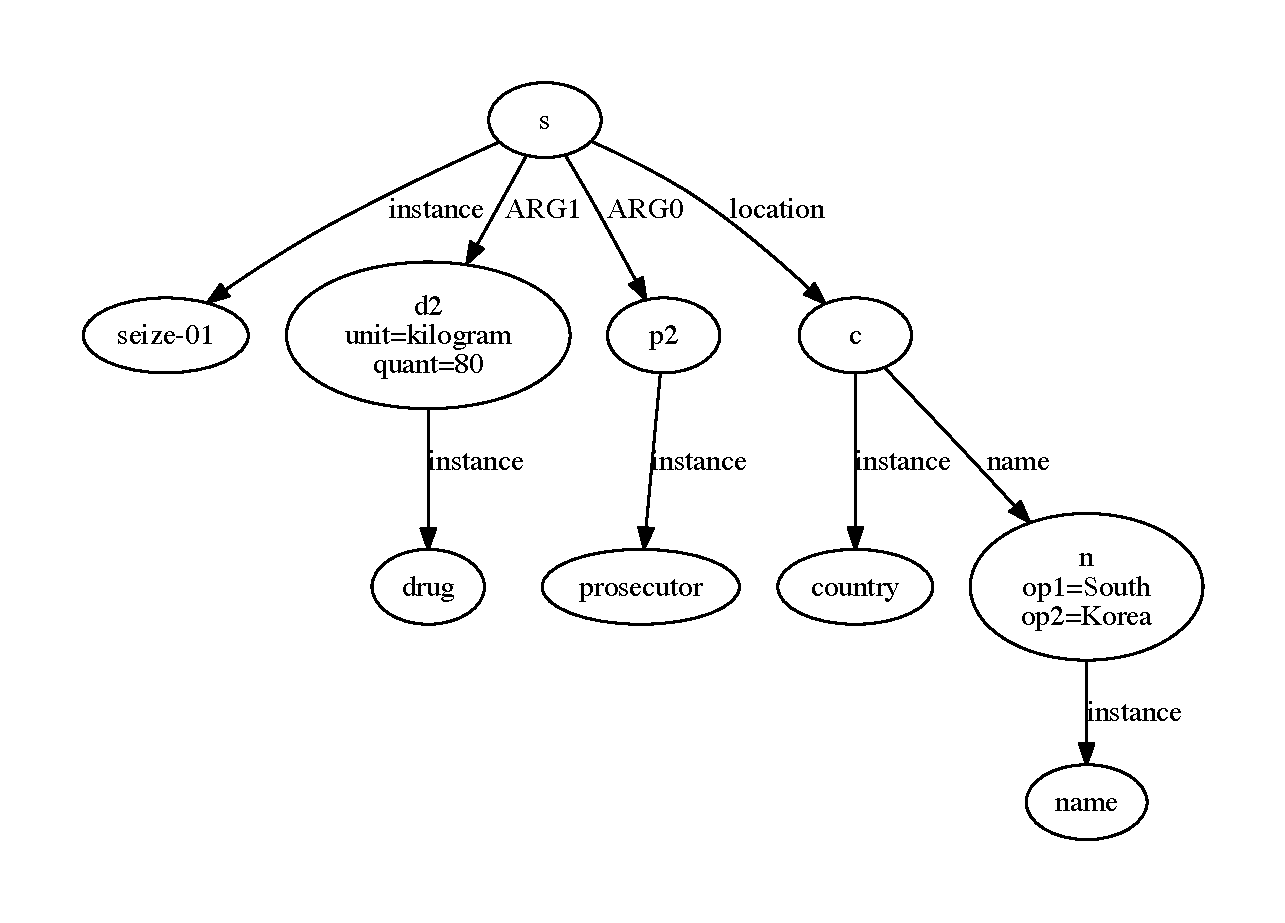
\includegraphics[width=\linewidth]{amr_example.pdf}
\label{fig:amr_example}
\caption{Example AMR}
\end{figure}

Our training set had 1676 ``paragraphs" of size $k=5$, and our test set had 214
paragraphs.

\section{Preprocessing}
Before we can feed our dataset through our featurizer and training/test pipeline, we have to apply various transformations to it: the first two are to ensure uniform sentence semantics and the third is to build our paragraph semantics.

\subsection{ARG-of Reversal}
The typical annotation for a sentence is the one shown in figure \ref{fig:amr_example}. However, due to the flattened textual representation of AMR, it is sometimes easier for annotators to add reversed edges. For example, in figure \ref{fig:amr_example}, instead of adding the edge: (`s', `p2', `ARG0'), they could have added (`p2', `s', `ARG0-of'), resulting in figure \ref{fig:amr_example_argof}. To fix this, we just reverse any such edge and change the label from `ARGN-of' to `ARGN'.

\begin{figure}
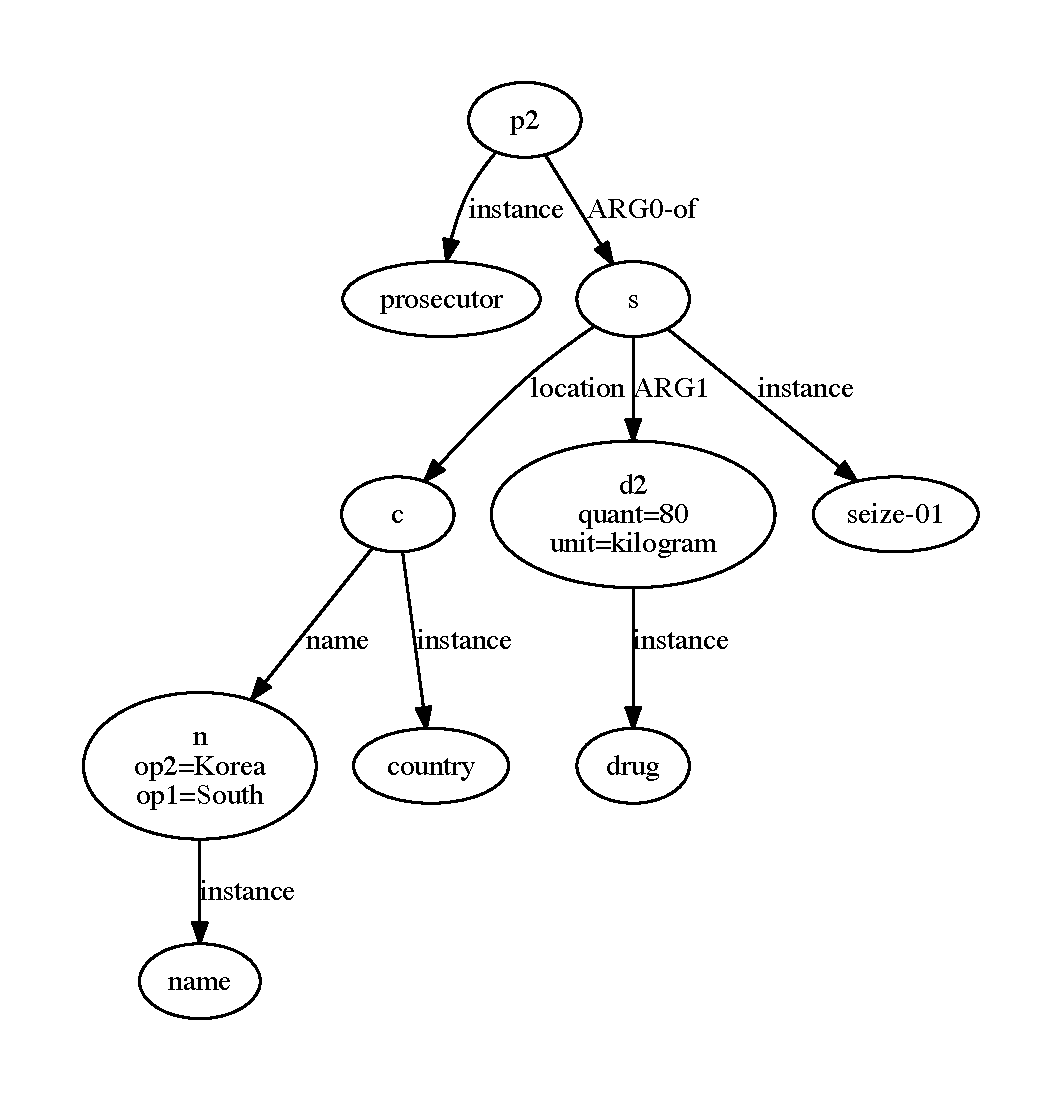
\includegraphics[width=\linewidth]{amr_example_argof.pdf}
\caption{AMR with Reversed Edge}
\label{fig:amr_example_argof}
\end{figure}

\subsection{Translation of `and' Semantics}
The next issue that we had to address in the sentence semantics was the way `and' is handled in AMR. For ease of annotation when `and' occurs in a sentence, an `and' instance is created with everything being `anded' together as its children. Then this `and' instance is used as the argument wherever one of the instances children would have gone before. For example, if instead our example sentence were ``A prosecutor in South Korea seized 80 kilograms of drugs and dozens of weapons.'', we would have the AMR graph shown in figure \ref{fig:amr_example_and}.

\begin{figure}
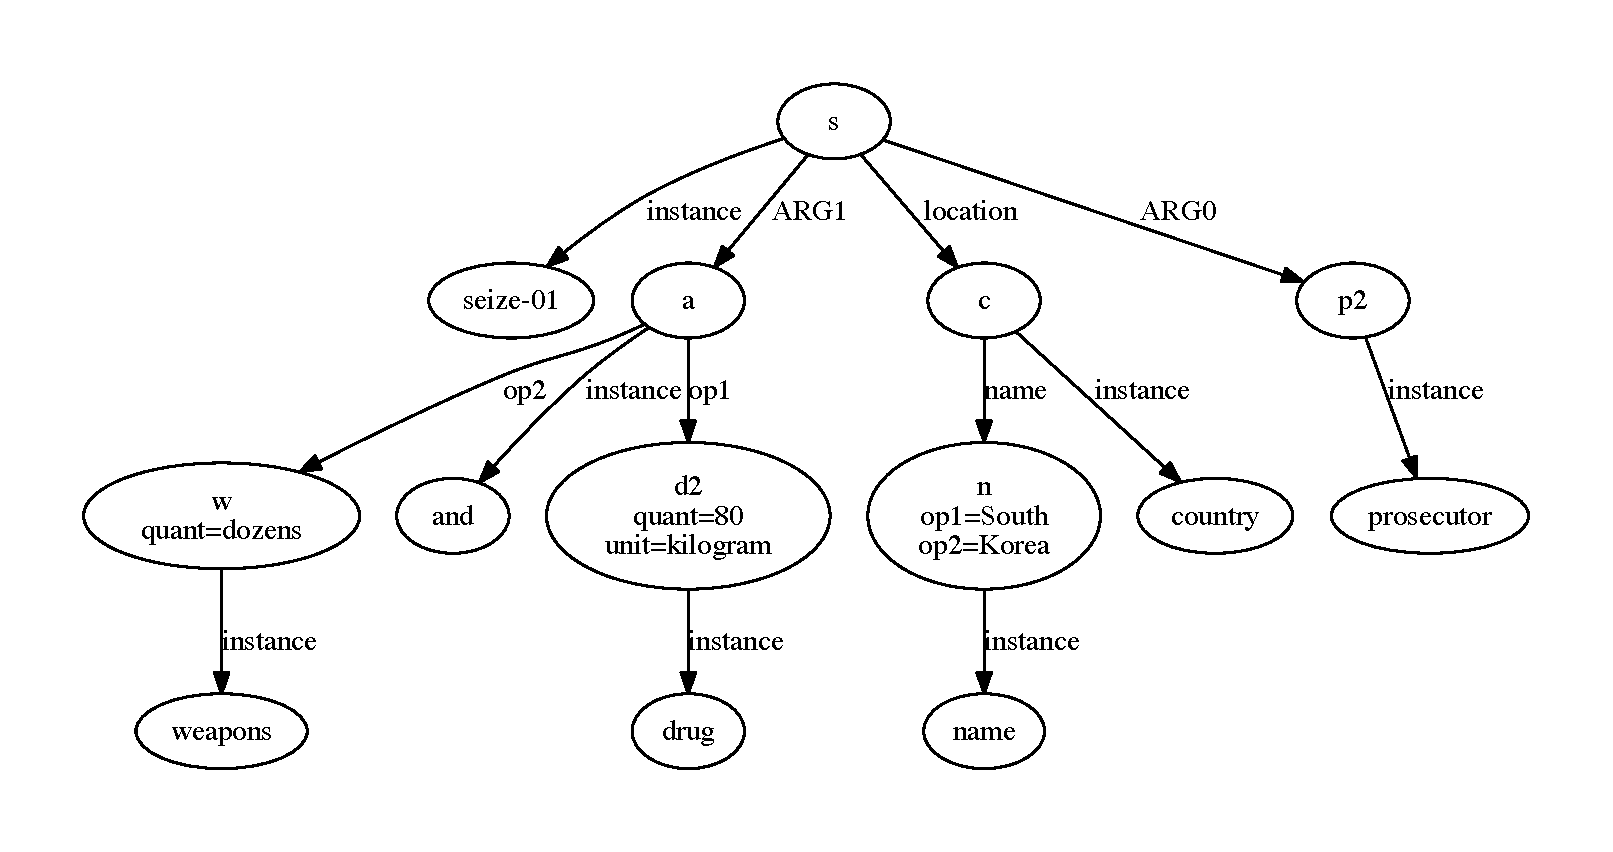
\includegraphics[width=\linewidth]{amr_example_and.pdf}
\caption{AMR with `and' Instance}
\label{fig:amr_example_and}
\end{figure}

While this is representation is not necessarily {\em wrong}, the choice to `and' these two entities together was syntactic, not semantic. A strictly semantic representation of this sentence should contain the information: there is a prosecutor, there are drugs, there are weapons, the prosecutor seized the drugs, and the prosecutor seized the weapons. In a generation process, this could be realized as one sentence (``A prosecutor in South Korea seized 80 kilograms of drugs and dozens of weapons.'') or two sentences (``A prosecutor in South Korea seized 80 kilograms of drugs. The prosecutor also seized dozens of weapons.''). Since we ultimately want to look at how information in paragraphs is grouped into sentences and then ordered, we need to translate these `and' semantics back to a strictly semantic representation; otherwise, we have already encoded some of our information grouping.

To recover the actual semantics from the `and' semantics, we must make N copies of each `and' instance, where N is the number of children of that `and' instance. Then, for each child, we must delete the copied `and' instance and replace it with the child. This algorithm is written formally in algorithm \ref{alg:translate_and_semantics}.

When we apply this algorithm to our semantic graph in figure \ref{fig:amr_example_and}, a new `seize-01' instance is made with the `drugs' instance as ARG1 and the `weapons' instance as ARG1 respectively. This resulting graph is shown in figure \ref{fig:amr_example_and_removed}.

\begin{algorithm}
\caption{Translate `and' Semantics}
\label{alg:translate_and_semantics}
\begin{algorithmic}[1]
%require: amr graph
\REQUIRE AMR Graph $G = (V, E)$

% While the graph still has and instances
\WHILE{$|G.and\_instances| > 0$}
    % and_instance = first and instance in topological ordering of G.and_instances
    \STATE $a \gets$ first and\_instance in topological ordering of $G$.and\_instances

    % S = subgraph formed by performing a breadth first search following parent edges from and_instance upwards to roots
    \STATE $S \gets$ subgraph formed by performing a breadth first search following parent edges from $a$ upwards to roots

    % for each child of the and instance
    \FOR{$c \in$ children($a$)}
        % copy S
        \STATE $S' \gets copy(S)$

        % replace and_instance in S with child
        \STATE replace $a$ with $c$ in $S'$

        % add copy to graph
        \STATE $G \gets G \cup S'$
    \ENDFOR
    % delete and_instance and S from graph
    \STATE remove $a$ and $S$ from $G$
\ENDWHILE
% return G
\RETURN $G$
\end{algorithmic}
\end{algorithm}

\begin{figure}
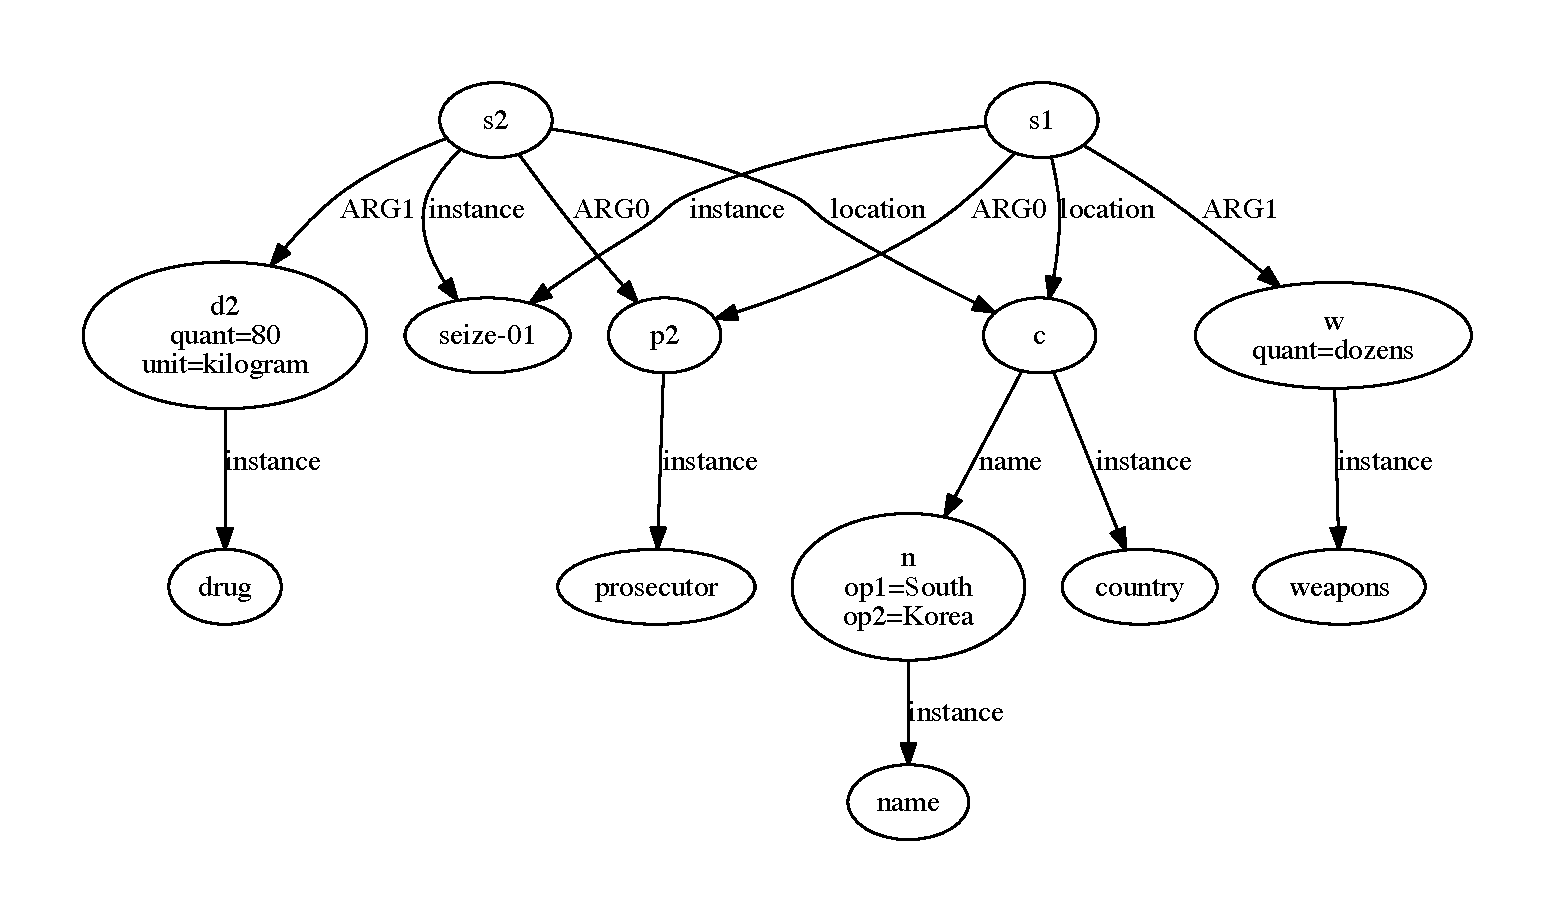
\includegraphics[width=\linewidth]{amr_example_and_removed.pdf}
\caption{AMR with Translated `and' Instance}
\label{fig:amr_example_and_removed}
\end{figure}

\subsection{Graph Merging}
After the semantic graphs have been preprocessed for each sentence, they have to be merged together to form paragraph semantic graphs. The only complication is deciding if two entities in separate sentences are the same. For example if we are merging the sentences ``The red dog chased the cat. Afterwards, the dog slept.'', the two dogs should be recognized as the same entity. However, if the sentences were ``The red dog chased the cat. The black dog slept.'', the two dogs should be recognized as separate. 

We define two nodes $u, v$ as {\b equivalent} if they are two `concept' nodes with the same label, or they have no conflicting attributes and no conflicting children. Formally:

\[
    equiv(u,v) = \left\{\begin{array}{lr}
    u.\text{label} = v.\text{label}, & u,v \text{ `concepts'} \\
    \forall k \text{ attribute of } u \text{ and } v, v.\text{attr}[k] = v.\text{attr}[k] \text{ } \land, & \text{else} \\
    \forall e,f \text{ childedge of } u,v \text{ with same label, } equiv(e.\text{child}, f.\text{child}) & \\
    \end{array}\right\}
\]

To merge two sentences, we use our node equivalence function in addition to algorithm \ref{alg:merge_graphs}. Since this algorithm returns a new, merged graph, we can continually apply it to a list of sentences as a reduction function, resulting in a semantic paragraph graph. Figure \ref{fig:amr_example_3_merged} shows the resultant semantic paragraph graph of the following piece of text: ``A prosecutor in South Korea seized 80 kilograms of drugs. The prosecutor disposed of the drugs. South Korean media stated the drugs originated from North Korea.'' We will continue to use this paragraph as an example throughout the paper.

The only issue of concern during graph merging is what to do when a node in one graph has multiple equivalent nodes in the second graph. This can be caused by annotation errors (i.e. a `name' attribute is annotated ``John F. Kennedy'' in one sentence and ``JFK'' in another) or underspecification (i.e. there are two dogs in the world and the next sentence simply refers to ``the dog''). When this happens, there is no clear resolution, so we drop the errant paragraph from our dataset.

\begin{algorithm}
\caption{Merge Two Sentence Semantic Graphs}
\label{alg:merge_graphs}
\begin{algorithmic}[1]
\REQUIRE Two AMR Graphs $G, H$

\FOR{$u \in H.\text{nodes}$}
    \STATE $equiv\_nodes \gets \{v \mid v \in G.\text{nodes} \land equiv(u,v)\}$
    \IF{$|equiv\_nodes| = 0$}
        \STATE $G.\text{nodes} \gets G.\text{nodes} \cup \{\text{safe\_rename}(G, u)\}$
    \ELSIF{$|equiv\_nodes| = 1$}
        \STATE $equiv\_nodes[0].\text{attr} \gets equiv\_nodes[0].\text{attr} \cup u.\text{attr}$
    \ELSE
        \STATE Raise Ambiguity Error
    \ENDIF
\ENDFOR

\STATE $G.\text{edges} \gets G.\text{edges} \cup H.\text{edges}$

\RETURN $G$
\end{algorithmic}
\end{algorithm}

\begin{figure}
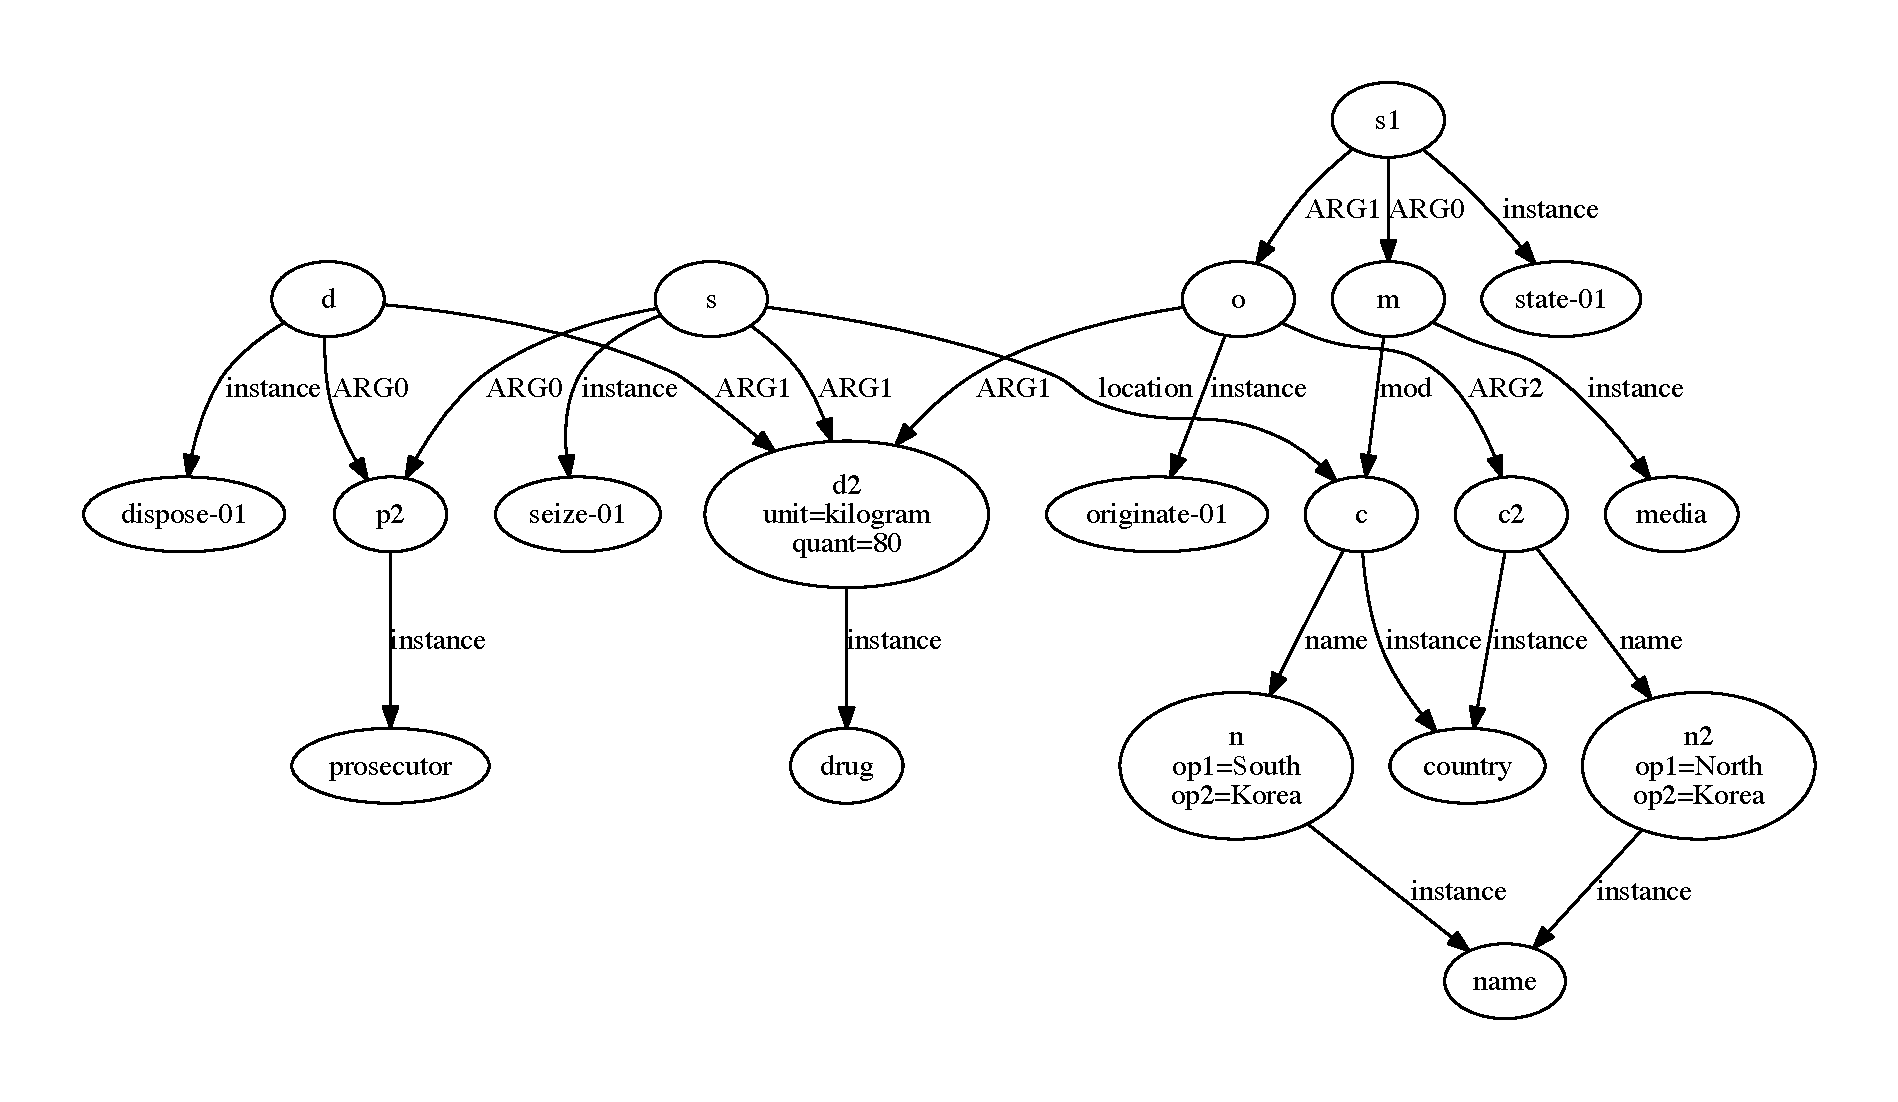
\includegraphics[width=\linewidth]{amr_example_3_merged.pdf}
\caption{Merged AMR Graph of Three Sentences}
\label{fig:amr_example_3_merged}
\end{figure}

\section{System Architecture}

From a high level, our system is a pipeline, which takes an AMR representation
of the information set that is to be communicated as input, and outputs a
sequence of AMR representations, which are the AMRs representing the sentences
containing all of the information in the information set.

To accomplish this task, we split the problem into two subproblems: (1)
subgraph selection and (2) subgraph ordering.

\subsection{Subgraph Selection}
\subsubsection{Problem Description}

Subgraph selection solves the problem of splitting an AMR graph into a set of
subgraphs which are optimal by some criterion, such that the union of the
subgraphs is the original graph. Said more plainly, the problem is to split the paragraph-level semantic graph 
into a set sentence-level semantic graphs.

There are $2^{|E|}$ subgraphs for a graph with $|E|$ edges. If we consider every set of $N$ subgraphs, we would have to consider $N^{2^{|E|}}$ sets of subgraphs! Obviously this is infeasible. Fortunately, we can exploit the natural language characteristics of a semantic graph to dramatically reduce the number of subgraph sets we have to consider. 

First, we define a {\em fact} in our semantic graph as the subgraph formed by performing a graph-traversal on a root of the graph (that is, a node with no parents). An example is shown in figure \ref{fig:amr_example_3_merged_s1_highlighted}. By design, the roots of an AMR graph will be verb instances. Therefore, we can intuitively think of the rooted graph traversal as a verb + the required graph pieces to fulfill the verb's arguments. A fact, then, is the the smallest piece of a graph that could be used to fully specify the semantics of a sentence during generation. Let $F$ refer to the set of facts in our graph.

\begin{figure}
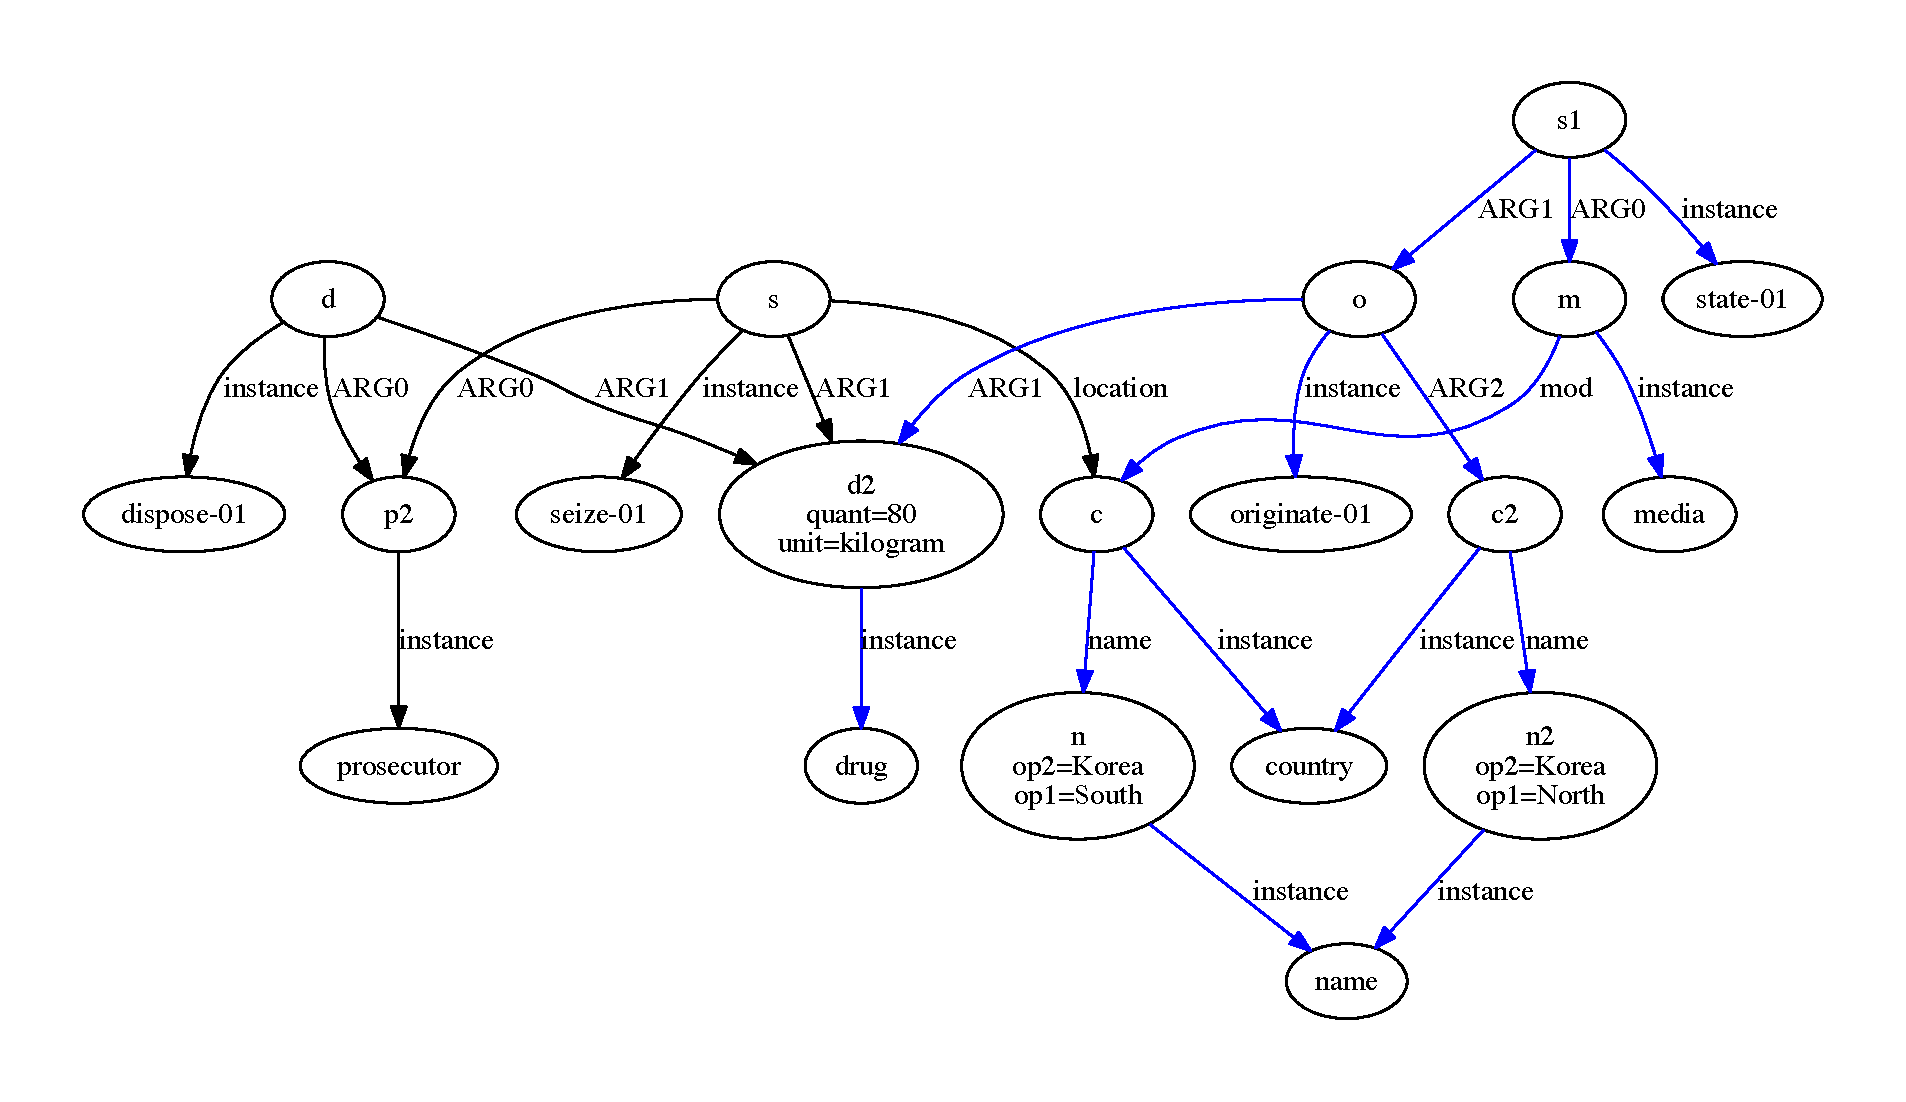
\includegraphics[width=\linewidth]{amr_example_3_merged_s1_highlighted.pdf}
\caption{AMR Graph with fact rooted by `s1' highlighted. Two other facts are present, rooted by `d' and `s'.}
\label{fig:amr_example_3_merged_s1_highlighted}
\end{figure}

Given $F$, our set of facts, and the assumption that we do not want to say the exact same thing twice, we can reduce our search-space to the set of partitions of $F$ from size 1 to $|F|$ (a single group with $|F|$ facts to $|F|$ groups each with 1 fact). The size of our candidate set is now given by $B_{|F|}$, where $B_i$ is the $i^{\text{th}}$ Bell number.

\subsubsection{Training}
Our problem then is to find the best partition from the $B_{|F|}$ candidates. To do this, we trained a scoring function using a logistic regression model with class-weighted instances. We assumed that the partitioning given by the sentences in a paragraph was the correct partitioning, and gave it a label of $1$. This means that we had only positive examples in the training set, so we added negative examples by sampling $k$ other partitions from the set of partitions, giving each a label of $0$.

Table \ref{tab:subgraph_selection_features} lists the features extracted for each candidate partition. To determine subgraph similarity, we used
Jaccard similarity, defined to be:
$$J(A,B) = \frac{\lvert A \cap B \rvert}{\lvert A \cup B \rvert}$$

\begin{table}[H]
\centering
\caption{Features used by subgraph partition scorer}
\label{tab:subgraph_selection_features}
\begin{tabular}{@{}ll@{}}
\toprule
\textbf{Feature}                      & \textbf{Weight} \\ \midrule
\# groups in partition                & 10.29970016     \\
\# groups in partition squared        & -1.17590317     \\
mean \# facts per partition           & 1.09239105      \\
max \# facts per partition            & -0.21350766     \\
min \# facts per partition            & 0.11910551      \\
std\_dev \# facts per partition       & 0.20101274      \\
mean pairwise subgraph similarity     & -18.66465415    \\
min pairwise subgraph similarity      & 1.77360275      \\
max pairwise subgraph similarity      & -0.38517871     \\
std\_dev pairwise subgraph similarity & -7.56089457     \\
mean pairwise verb set similarity     & -1.02945557     \\
min pairwise verb set similarity      & 0.04030027      \\
max pairwise verb set similarity      & 0.89961397      \\
std\_dev pairwise verb set similarity & -0.17388411     \\ \bottomrule
\end{tabular}
\end{table}

\subsubsection{Test}

\begin{table}[H]
\centering
\caption{Evaluation Metrics for Subgraph Selection Classifier}
\label{tab:subgraph_selection_eval}
\begin{tabular}{@{}lllll@{}}
\toprule
\textbf{Precision} & \textbf{Recall} & \textbf{f1-score} & \textbf{auc} & \textbf{support} \\ \midrule
0.93               & 0.93            & 0.93              & 0.98         & 428              \\ \bottomrule
\end{tabular}
\end{table}

\subsection{Subgraph Ordering}

Once we have split a merged graph into a partition of $p$ sentences, there are
$s!$ ways to order the sentences. Ideally, there exists some ordering of the
sentences that communicates the ideas of the merged graph in the best possible
way. Subgraph ordering is the problem of finding this optimal ordering.

Once again, we assumed that the ordering of sentences in the dataset was the
optimal ordering for that paragraph, so we needed to create non-optimal
examples to train on. This was done by randomly reordering the sentences for
$k=20$ reorderings for each paragraph.

We trained a Ridge regression model on the dataset. For the labels of the
training examples, we used the unnormalized Kendall's tau coefficient to
determine the distance between a given ordering and the optimal.

As noted in Related Work, our ordering model does not require the number of
sentences to be fixed to a particular value. If it were to impose such a
requirement, then the subgraph selection, which is further upstream in our
pipeline, may not be able to find its optimal partitioning simply because it
was a partitioning into a different number of sentences. As a result, our model
could not rely on any features that deal with particular sentences (e.g. the
similarity between the second and fifth sentences). So, we tried to use
features that would generalize to paragraphs of any length, but would still
vary with the ordering of those sentences within the paragraph, and all
features had to be summarized (mean, standard deviation, min, max) over the
paragraph. Features included the Jaccard similarity between adjancent
sentences, between sentences that are two sentences apart, and the Jaccard
similarity between the union of adjacent sentences and the overall paragraph.

\subsection{Discrete Optimization}

In both subproblems, we trained classifiers which assign a score to how ``good"
an instance is with regard to that problem. So, to find the best instance, we
could just enumerate all possible permutations or combinations of the input,
and select the instance which maximizes (or, in the case of subgraph ordering,
minimizes) the classifier's score. However, in the case of subgraph selection,
for a paragraph of $n$ facts, there are $O(2^n)$ possible partitions. In the
case of subgraph ordering, for a paragraph of $n$ sentences, there are $O(n!)$
possible orderings. Neither of these are very computationally efficient, so we
perform discrete optimization to approach an optimal solution, rather than
enumerating all possible inputs. It is worth noting that in practice, this is
more of a problem for the subgraph selection module, since the partitions
returned by the subgraph selector are generally not too large, so $n$ for the
subgraph orderer is not too bad.

For discrete optimization, we implemented a greedy search procedure as follows:
\begin{algorithm}
\caption{Greedy search procedure}
\label{greedy_search_alg}
\begin{algorithmic}
\STATE Input: $s$ // start state \\
\STATE Input: $classifier$ \\
\STATE $Q \gets [s]$ // queue of states to visit \\
\STATE $opt, optv, oldoptv \gets null, 0, 1$
\WHILE{$Q\neq\emptyset$ and $optv \neq oldoptv$}
    \STATE $S \gets \{s: s \in Q \}$
    \STATE $Q \gets \emptyset$
    \STATE $oldoptv \gets optv$
    \FORALL{$s \in S$}
        \STATE $N \gets neighbors(s)$\\
        \STATE Add all elements of $N$ to $Q$\\
        \IF{$classifier.score(s) > optv$}
            \STATE $opt, optv \gets s, classifier.score(s)$\\
        \ENDIF
    \ENDFOR
\ENDWHILE
\end{algorithmic}
\end{algorithm}

Additionally, we used a simulated annealing approach, but only for the
subgraph ordering problem.

\section{Evaluation of Scoring Modules}
\subsection{Subgraph Selection}
\subsection{Subgraph Ordering}

\section{Experiments}

\section{Conclusion and Future Work}

\pagebreak
\bibliographystyle{acm}
\bibliography{paper}
\end{document}
